\documentclass[a4paper,12pt]{article}
\usepackage{fullpage}
\usepackage{amsmath}
\usepackage{graphicx}
\usepackage{subfig}
\usepackage{bm}
\usepackage{amssymb}
\usepackage{fixltx2e}
\usepackage[nodisplayskipstretch]{setspace}
\usepackage{etoolbox}

\usepackage[margin=0.75in]{geometry}

\BeforeBeginEnvironment{equation}{\begin{singlespace}}
\AfterEndEnvironment{equation}{\end{singlespace}\noindent\ignorespaces}
%\BeforeBeginEnvironment{align}{\begin{singlespace}}
%\AfterEndEnvironment{align}{\end{singlespace}\noindent\ignorespaces}
%\BeforeBeginEnvironment{eqnarray}{\begin{singlespace}}
%\AfterEndEnvironment{eqnarray}{\end{singlespace}\noindent\ignorespaces}

\usepackage[compact]{titlesec}
\titlespacing{\section}{0pt}{*0}{*0}
\titlespacing{\subsection}{0pt}{*0}{*0}
\titlespacing{\subsubsection}{0pt}{*0}{*0}

\setlength{\abovedisplayskip}{0pt}
\setlength{\belowdisplayskip}{0pt}
\setlength{\abovedisplayshortskip}{0pt}
\setlength{\belowdisplayshortskip}{0pt}

\allowdisplaybreaks

\renewcommand{\vec}[1]{\boldsymbol{\mathbf{#1}}}

\begin{document}

%\begin{flushright}
%Dillon Wong \\
%\end{flushright}

\begin{center}
\mbox{} \\
{ \large An Introduction to the Quantum Spin Hall Effect}
\end{center}

\doublespacing

In a strong magnetic field, two dimensional (2D) electron systems exhibit the integer quantum Hall effect, which consists of an insulating state and edge modes with Hall conductance $\sigma_{xy}=ne^2/h$, where $n$ is an integer.  The quantum Hall state is fundamentally different from that of an ordinary insulator in that the electronic structure of a quantum Hall insulator cannot be continuously deformed into that of a ``trivial insulator" without closing the energy gap.  The quantum spin Hall (QSH) effect is also an insulating state with conducting edge channels.  However, unlike the quantum Hall effect, the QSH effect occurs in the absence of a magnetic field.  This paper will discuss the QSH effect, starting with the Haldane model for a quantum Hall system.  We will show that the Hall conductivity for the Haldane model is nonzero, and we will apply the Haldane model to Kane and Mele's model for a QSH insulator.

\begin{section}{The Berry Phase}

Let's first review the concept of a Berry phase.  When a vector is parallel transported in a loop on a curved surface, the vector will acquire an anholonomy angle.  Analogously, in quantum mechanics, a state indexed by a continuous set of parameters $\vec{R}$ that is adiabatically evolved along a closed parametrization of $\vec{R}$ will acquire a Berry phase \cite{griffiths}
\begin{equation}
\gamma_n=i \oint \langle n, \vec{R} | \nabla_{\vec{R}} | n, \vec{R} \rangle \cdot d\vec{R}
\end{equation}
To understand the curved surface on which $| n, \vec{R} \rangle$ is being parallel transported would require the concept of a fiber bundle, which is outside the scope of this paper.  The quantity in the integrand $\vec{A}_n(\vec{R})=i \langle n, \vec{R} | \nabla_{\vec{R}} | n, \vec{R} \rangle$ is known as the Berry connection, which is not gauge invariant.  We can construct a gauge invariant quantity known as the Berry curvature
\begin{equation}
\vec{\Omega}_n(\vec{R})=i \nabla_{\vec{R}} \times \langle n, \vec{R} | \nabla_{\vec{R}} | n, \vec{R} \rangle
\end{equation}
Then, using Stoke's Theorem, we can write the Berry phase as
\begin{equation}
\gamma_n=\int_S \vec{\Omega}_n(\vec{R}) \cdot d\vec{S}
\end{equation}
where $S$ is a surface whose boundary is the closed curve parameterized by $\vec{R}$.  Given eigenstates of energy $E_n(\vec{R})$ of a Hamiltonian $H(\vec{R})$ parameterized by $\vec{R}$, the Berry curvature can easily be rewritten in another form \cite{bernevig}
\begin{equation}\label{eq:curvature}
\vec{\Omega}_n(\vec{R})=- \text{Im} \sum_{m \ne n}{\frac{\langle n, \vec{R} | (\nabla_{\vec{R}} H) | m, \vec{R} \rangle \times \langle m, \vec{R} | (\nabla_{\vec{R}} H) | n, \vec{R} \rangle}{(E_m(\vec{R})-E_n(\vec{R}))^2}}
\end{equation}
This form is useful because one can immediately see that the sum of the Berry curvatures of all energy levels is zero.

We can gauge away the Berry phase if we replace $i \nabla_{\vec{R}}$ by $i \nabla_{\vec{R}}+\vec{A}_n(\vec{R})$ everywhere in the Hamiltonian \cite{louie}.  In this sense, $\vec{A}_n(\vec{R})$ is similar to the magnetic vector potential, and since $\vec{\Omega}_n(\vec{R}) = \nabla_{\vec{R}} \times \vec{A}_n(\vec{R})$, the Berry curvature acts like a magnetic field in the parameter space of $\vec{R}$.  If we imagine a crystalline solid, we can let the parameter $\vec{R}$ be the crystal momentum $\vec{k}$ of Bloch states.  Then, we can think of the Berry curvature as a k-space magnetic field, and so the semiclassical equations of motion are \cite{luttinger}
\begin{eqnarray}
\hbar \frac{d\vec{k}}{dt}&=&-e \left[ \vec{E}+\vec{v} \times \vec{B} \right] \\
\hbar \vec{v}&=&\nabla_{\vec{k}}E_n(\vec{k})+e \vec{E} \times \vec{\Omega}_n(\vec{k})
\end{eqnarray}
where $e=|e|$, $\vec{v}$ is velocity, $\vec{E}$ is an applied electric field, and $\vec{B}$ is a magnetic field.  To get the current, we sum $\vec{v}$ over all filled states.  For a full band, summing $\nabla_{\vec{k}}E_n(\vec{k})$ will yield zero, but the ``anomalous velocity" $e \vec{E} \times \vec{\Omega}_n(\vec{k})$ does not necessarily add to zero.  Also notice that the anomalous velocity is perpendicular to $\vec{E}$, so it contributes to $\sigma_{xy}$.

To be more exact, we can compute the Hall conductance for a 2D insulator directly using the Kubo-Greenwood Formula \cite{tknn}.  The Kubo-Greenwood Formula is almost of the same form as the Berry curvature given in Eq. (\ref{eq:curvature}), so it does not take much effort to show that the Hall conductance is the integral of the Berry curvature over all filled states
\begin{equation}
\sigma_{xy}=\frac{e^2}{h} \frac{1}{2 \pi} \sum_n \int_{BZ} dk_x dk_y \Omega_{xy}(\vec{k})
\end{equation}
\begin{equation}
\Omega_{xy}(\vec{k})=\frac{\partial A_y(\vec{k})}{\partial k_x} - \frac{\partial A_x(\vec{k})}{\partial k_y}
\end{equation}
where $BZ$ is the Brillouin zone.  The Berry curvature $\Omega_{xy}(\vec{k})$ depends on the band index $n$, and the sum over $n$ is taken only over filled bands.  Another way to derive this relationship between Hall conductance and Berry curvature is to treat the applied electric field as a vector potential $-\vec{E}t$ in time-dependent perturbation theory \cite{berry_electronic}.

\end{section}

\begin{section}{A Honeycomb Lattice}

\begin{figure}[h!]
\centering
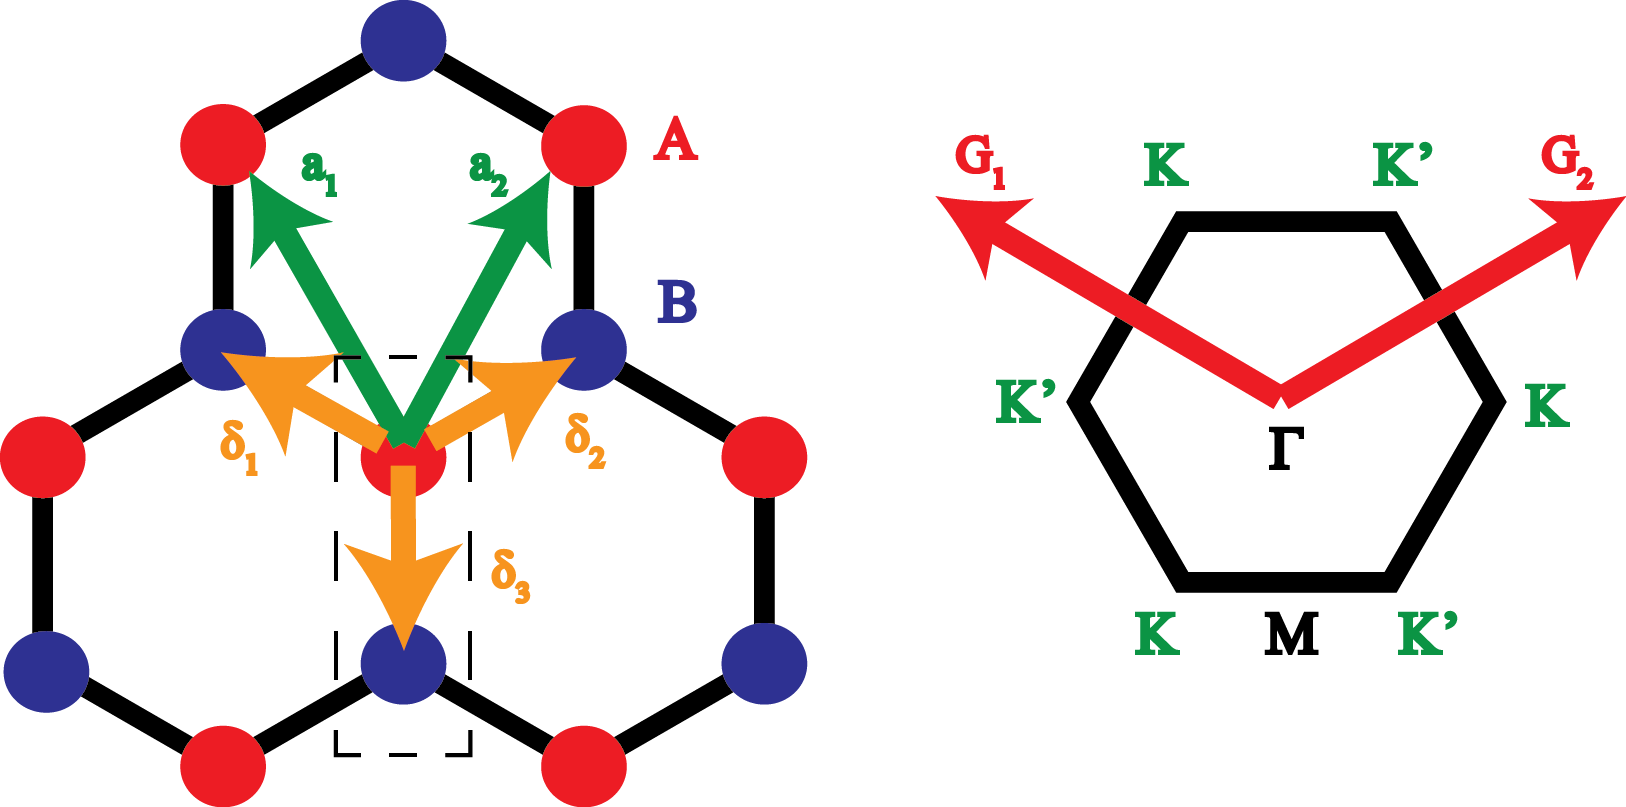
\includegraphics[width=70mm,keepaspectratio=true]{honeycomb_primitive_cell.png}
\caption{Honeycomb Lattice and Brillouin Zone}\label{fig:honeycomb}
\end{figure}

The Haldane model involves a honeycomb lattice, so lets introduce the theory of electrons on such a lattice \cite{katsnelson}.  The honeycomb lattice is made of two interpenetrating triangular sublattices, hereby denoted as the $A$ and $B$ sublattices (see Fig. \ref{fig:honeycomb}).  Each triangular sublattice can be constructed by the primitive lattice vectors
\begin{equation}
\vec{a}_1 = a \left( -\frac{\sqrt{3}}{2}, \frac{3}{2} \right), \text{ }
\vec{a}_2 = a \left( \frac{\sqrt{3}}{2}, \frac{3}{2} \right)
\end{equation}
where $a$ is the distance between a point on the $A$ sublattice and its nearest neighbors on the $B$ sublattice.  The vectors between a point and its nearest neighbors are
\begin{equation}
\vec{\delta}_1 = a \left( -\frac{\sqrt{3}}{2}, \frac{1}{2} \right), \text{ }
\vec{\delta}_2 = a \left( \frac{\sqrt{3}}{2}, \frac{1}{2} \right), \text{ }
\vec{\delta}_3 = a \left( 0, -1 \right)
\end{equation}
Define a unit cell to encompass a point on $A$ and its nearest neighbor on $B$ at $\vec{\delta}_3$. The reciprocal lattice vectors are
\begin{equation}
\vec{G}_1 = \frac{2 \pi}{a} \left( -\frac{1}{\sqrt{3}}, \frac{1}{3} \right), \text{ }
\vec{G}_2 = \frac{2 \pi}{a} \left( \frac{1}{\sqrt{3}}, \frac{1}{3} \right)
\end{equation}
The Brillouin Zone for a triangular lattice is a hexagon with high symmetry points $K$ and $K'$ on its corners:
\begin{equation}
\vec{K} = \frac{2 \pi}{a} \left(\frac{2}{3 \sqrt{3}}, 0 \right), \text{ }
\vec{K}' = \frac{2 \pi}{a} \left( -\frac{2}{3 \sqrt{3}}, 0 \right)
\end{equation}
Lets now consider a tight binding model with nearest neighbor hopping amplitude $t$
\begin{equation}
\label{eq:graphene_hamiltonian}
H= U \sum_i a_i^\dagger a_i- U \sum_j b_j^\dagger b_j - t \sum_{\langle i,j \rangle} \left( a_i^\dagger b_j + \text{h.c.} \right)
\end{equation}
where $a_i^\dagger$ and $a_i$ are the creation and annihilation operators for site $i$ on sublattice $A$ (and similarly, $b_j^\dagger$ and $b_j$ are for $B$).  $U$ is half the energy difference between an electron sitting on an atom of sublattice $B$ as opposed to $A$. \\
Let $|A,\vec{r} \rangle$ represent a Wannier function localized on the $A$ site in the unit cell at $\vec{r}$.  Then,
\begin{equation}
H|A,\vec{r} \rangle = U|A,\vec{r} \rangle -t \left( |B,\vec{r}+\vec{a}_1 \rangle + |B,\vec{r}+\vec{a}_2 \rangle + |B,\vec{r} \rangle \right)
\end{equation}
And similarly for $|B,\vec{r} \rangle$ localized at $B$ in the unit cell at $\vec{r}$:
\begin{equation}
H|B,\vec{r} \rangle = -U|B,\vec{r} \rangle -t \left( |A,\vec{r}-\vec{a}_1 \rangle + |A,\vec{r}-\vec{a}_2 \rangle + |A,\vec{r} \rangle \right)
\end{equation}
Define Bloch states
\begin{eqnarray}
|A, \vec{k} \rangle = \sum_{\vec{r}} e^{i \vec{k} \cdot \vec{r}} |A,\vec{r} \rangle \label{eq:bloch_a} \\
|B, \vec{k} \rangle = \sum_{\vec{r}} e^{i \vec{k} \cdot \vec{r}} |B,\vec{r} \label{eq:bloch_b} \rangle
\end{eqnarray}
Applying the Hamiltonian on these Bloch states,
\begin{eqnarray}
H|A,\vec{k} \rangle % &=& U|A,\vec{k} \rangle -t \sum_{\vec{r}}  e^{i \vec{k} \cdot \vec{r}} \left( |B,\vec{r}+\vec{a}_1 \rangle + |B,\vec{r}+\vec{a}_2 \rangle + |B,\vec{r} \rangle \right) \nonumber \\
 &=& U|A,\vec{k} \rangle -t \left( e^{-i \vec{k} \cdot \vec{a}_1}+e^{-i \vec{k} \cdot \vec{a}_2} +1 \right)|B, \vec{k} \rangle \\
H|B,\vec{k} \rangle &=& -U|B,\vec{k} \rangle - t \left( e^{i \vec{k} \cdot \vec{a}_1}+e^{i \vec{k} \cdot \vec{a}_2} +1 \right)|A, \vec{k} \rangle
\end{eqnarray}
Clearly, the Hamiltonian for each $\vec{k}$ subspace can be represented by the matrix
\begin{equation}
H(\vec{k})= -t \left(
\begin{array}{cc}
U & e^{-i \vec{k} \cdot \vec{a}_1}+e^{-i \vec{k} \cdot \vec{a}_2} +1  \\
e^{i \vec{k} \cdot \vec{a}_1}+e^{i \vec{k} \cdot \vec{a}_2} +1 & -U
\end{array}
\right)
\end{equation}
We can rewrite the Hamiltonian in terms of the Pauli matrices $\sigma_x$, $\sigma_y$, and $\sigma_z$ by defining
\begin{eqnarray}
X(\vec{k}) &=& -t \left[ 1+ \cos \left( \frac{\sqrt{3}}{2}k_x a - \frac{3}{2}k_y a \right) + \cos \left( -\frac{\sqrt{3}}{2}k_x a - \frac{3}{2}k_y a \right) \right] \\
Y(\vec{k}) &=& t \left[ \sin \left( \frac{\sqrt{3}}{2}k_x a - \frac{3}{2}k_y a \right) + \sin \left( -\frac{\sqrt{3}}{2}k_x a - \frac{3}{2}k_y a \right) \right] \\
Z(\vec{k}) &=& U
\end{eqnarray}
so that $H(\vec{k})=X(\vec{k}) \sigma_x + Y(\vec{k}) \sigma_y+Z(\vec{k}) \sigma_z$ and $E(\vec{k})=\pm \sqrt{X(\vec{k})^2+Y(\vec{k})^2+Z(\vec{k})^2}$ for all $\vec{k}$ in the Brillouin Zone.  We can obtain the low energy electronic structure by expanding $X(\vec{k})$ and $Y(\vec{k})$ around the $K$ point (i.e., let $\vec{k}=\vec{K}+\vec{q}$): $X(\vec{k}) \approx \frac{3at}{2} q_x$, $Y(\vec{k}) \approx \frac{3at}{2} q_y$.
%\begin{equation}
%X(\vec{k}) \approx \frac{3at}{2} q_x, \text{ }
%Y(\vec{k}) \approx \frac{3at}{2} q_y
%\end{equation}
Thus,
\begin{equation}
H(\vec{K}+\vec{q})=\hbar v_F \left( q_x \sigma_x + q_y \sigma_y \right) + U \sigma_z
\end{equation}
where $v_F=\frac{3at}{2\hbar}$.  This is the two-dimensional Dirac Equation with mass $U$ and the speed of light replaced by $v_F$.  For a similar expansion near $K'$: $H(\vec{K'}+\vec{q})=\hbar v_F \left( - q_x \sigma_x + q_y \sigma_y \right) + U \sigma_z$.
%\begin{equation}
%H(\vec{K'}+\vec{q})=\hbar v_F \left( - q_x \sigma_x + q_y \sigma_y \right) + U \sigma_z
%\end{equation}

Graphene is similar to this tight binding model in that the electrons in graphene hop between the out-of-plane p orbitals \cite{castro_neto}.  For graphene, there is no energy difference between $A$ and $B$, so $U=0$.  Thus, $E=\pm \hbar v_F q$, so graphene is not gapped.  On the other hand, $U \ne 0$ for hexagonal boron nitride (h-BN), so it has a gap at $K$ and $K'$.

\end{section}

\begin{section}{A Trivial Insulator}

Let $\vec{d}(\vec{k})=(d_x,d_y,d_z)=(X(\vec{k}),Y(\vec{k}),Z(\vec{k}))$.  Parameterize $\vec{d}(\vec{k})$ in spherical coordinates $\vec{d}(\vec{k})=|\vec{d}(\vec{k})| (\sin{\theta} \cos{\phi},\sin{\theta} \sin{\phi}, \cos{\phi})$, where $\theta$ and $\phi$ depend on $\vec{k}$, and $|\vec{d}(\vec{k})|=E(\vec{k})$.  Then, the Hamiltonian is
\begin{equation}
H(\vec{k})=\vec{d}(\vec{k}) \cdot \vec{\sigma}=|\vec{d}(\vec{k})| \left(
\begin{array}{cc}
\cos{\theta} & \sin{\theta} e^{-i \phi}  \\
\sin{\theta} e^{i \phi} & -\cos{\theta}
\end{array}
\right)
\end{equation}
The eigenvectors of this matrix are \cite{berry_electronic}
\begin{equation}
| \vec{k}, - \rangle = \left(
\begin{array}{c}
\sin{\frac{\theta}{2}} e^{-i \phi} \\
-\cos{\frac{\theta}{2}}
\end{array}
\right), \text{ }
| \vec{k}, + \rangle = \left(
\begin{array}{c}
\cos{\frac{\theta}{2}} e^{-i \phi} \\
\sin{\frac{\theta}{2}}
\end{array}
\right)
\end{equation}
The state $| \vec{k}, - \rangle$ has lower energy than $| \vec{k}, + \rangle$.  We can calculate the Berry curvature with respect to parameters $\theta$ and $\phi$.  We only need to calculate this for the lower energy state because the curvatures must sum to zero:
\begin{eqnarray}
A_{\theta} = \langle \vec{k}, - | \frac{\partial}{\partial \theta} | \vec{k}, - \rangle = 0 \\
A_{\phi} = \langle \vec{k}, - | \frac{\partial}{\partial \phi} | \vec{k}, - \rangle = \sin^2 \frac{\theta}{2} \\
\Omega_{\theta,\phi} = \frac{\partial}{\partial \theta} A_{\phi} - \frac{\partial}{\partial \phi} A_{\theta} = \frac{1}{2} \sin{\theta}
\end{eqnarray}
We can convert this to a Berry curvature with respect to $k_x$ and $k_y$ by multiplying by the Jacobian of the transformation between $(\theta,\phi)$ and $(k_x,k_y)$:
\begin{equation}
\Omega_{k_x,k_y}=\Omega_{\theta,\phi} \left[ \frac{\partial \theta}{\partial k_x} \frac{\partial \phi}{\partial k_y} - \frac{\partial \phi}{\partial k_x} \frac{\partial \theta}{\partial k_y} \right]
\end{equation}
Thus, the Hall conductance will be
\begin{equation}
\sigma_{xy}=\frac{e^2}{h} \frac{1}{4 \pi} \int_{BZ} dk_x dk_y \sin{\theta} \left[ \frac{\partial \theta}{\partial k_x} \frac{\partial \phi}{\partial k_y} - \frac{\partial \phi}{\partial k_x} \frac{\partial \theta}{\partial k_y} \right]
\label{eq:hall_sine}
\end{equation}
After another change of variables \cite{dirac_materials}
\begin{equation}
\sigma_{xy}=\frac{e^2}{h} \frac{1}{2 \pi} \int_{BZ} \frac{1}{2} \frac{\vec{d}(\vec{k})}{|\vec{d}(\vec{k})|^3}\cdot \left( \frac{\partial \vec{d}(\vec{k})}{\partial k_x} \times \frac{\partial \vec{d}(\vec{k})}{\partial k_y}\right) dk_x dk_y
\label{eq:degree}
\end{equation}
How do we interpret the above expression?  If $H=\vec{d}(\vec{k}) \cdot \vec{\sigma}$, then $\nabla_{\vec{d}({\vec{k})}}H=\vec{\sigma}$.  Plugging into Eq. (\ref{eq:curvature}), for $\vec{R}=\vec{d}(\vec{k})$ and the lower energy state
\begin{equation}
\vec{\Omega}_-(\vec{d}(\vec{k}))=\frac{1}{2} \frac{\vec{d}(\vec{k})}{|\vec{d}(\vec{k})|^3}
\end{equation}
The rest of the integrand is the unit normal to $S$, the surface in $\mathbb{R}^3$ parametrized by $\vec{d}(\vec{k})$ as $\vec{k}$ sweeps over the entire Brillouin zone.  In other words, $S$ is the image of the map $\vec{k} \rightarrow \vec{d}(\vec{k})$.  We will discuss the importance of this later, but as an aside, the Gauss-Bonnet Theorem asserts that the surface integral of a curvature is a topological invariant.  For now, lets return to Eq. (\ref{eq:hall_sine}), which can be rewritten as
\begin{equation}
\sigma_{xy}=-\frac{e^2}{h} \frac{1}{4 \pi} \int_{BZ} dk_x dk_y \left[ \frac{\partial \left( \cos{\theta} \frac{\partial \phi}{\partial k_y} \right)}{\partial k_x} - \frac{\partial \left( \cos{\theta} \frac{\partial \phi}{\partial k_x} \right)}{\partial k_y} \right]
\end{equation}
Naively, this integral is zero because the Brillouin zone has the topology of a closed torus.  However, that is not necessarily true because the integrand contains $\nabla_{\vec{k}} \phi$, which has singularities at $\theta=0$ and $\theta=\pi$, the north and south poles of a Bloch sphere.  Thus, using Green's Theorem, the Hall conductance can be written as the sum of line integrals around points in the Brillouin zone where $\theta=0$ and $\theta=\pi$:
\begin{equation}
\sigma_{xy}=-\frac{e^2}{h} \frac{1}{4 \pi} \lim_{\epsilon \rightarrow 0} \sum_{\theta=0,\pi} \oint_{C(\epsilon)} \cos(\theta) \nabla_{\vec{k}} \phi \cdot d\vec{k}
\end{equation}
where $C(\epsilon)$ is an infinitesimally small circle around the singularity.  If we were to do a more careful analysis, we would find that a nonzero Hall conductance comes from an obstruction of Stokes' Theorem over the Brillouin zone due to the fact that we cannot define a smooth gauge for all the wavefunctions.

Does our model for a honeycomb lattice have a nonzero Hall conductivity?  We will now show that the answer is no.  The angles $\theta=0$ and $\theta=\pi$ occur at the $K$ and $K'$ points.  We can write the Hamiltonian as $H=\xi q_x \sigma_x + q_y \sigma_y + M \sigma_z$, where we let $M=Z=U$, $\xi = \pm 1$ depending on whether we are at $K$ or $K'$, and $\hbar v_F = 1$ for convenience.  We can also shift $q_x$ and $q_y$ to $k_x$ and $k_y$, so the Hamiltonian becomes $H=\xi k_x \sigma_x + k_y \sigma_y + M \sigma_z$.  
%\begin{equation}
%H=\xi k_x \sigma_x + k_y \sigma_y + M \sigma_z
%\end{equation}
Then, $\cos{\theta}=M/|\vec{d}(\vec{k})|=M/\sqrt{k_x^2+k_y^2+M^2}$.  Since $\epsilon \rightarrow 0$, $\cos{\theta}=\text{sign}(M)$.  The closed loop integral of $\nabla_{\vec{k}} \phi$ can easily be evaluated explicitly, but there is no need because $\phi$ is an angle whose direction clockwise or counterclockwise is controlled by $\xi$. Thus, $\oint \nabla_{\vec{k}} \phi \cdot d\vec{k}=2\pi \xi$.  Putting it all together,
\begin{equation}
\sigma_{xy}=-\frac{e^2}{h} \sum_{\theta=0,\pi} \frac{\xi}{2} \text{ sign}(M) = \frac{e^2}{h} \left[ \frac{1}{2} \left( \text{sign}(Z(\vec{k}=\vec{K'})) - \text{sign}(Z(\vec{k}=\vec{K}) ) \right) \right]
\label{eq:sign_of_mass}
\end{equation}
Since $Z(\vec{k}=\vec{K})=Z(\vec{k}=\vec{K'})=M$ in our model, $\sigma_{xy}=0$.  The system described by the Hamiltonian in Eq. (\ref{eq:graphene_hamiltonian}) is an example of a trivial insulator.  A trivial insulator is a system whose Hamiltonian can be continuously deformed into the vacuum without closing the energy gap, and thus, a trivial insulator does not have quantized conductive edge states.

\end{section}

\begin{section}{The Haldane Model}

Now we can finally discuss the Haldane model.  Haldane considers a honeycomb lattice in a spatially modulated magnetic field \cite{haldane_prl}.  The magnetic field is arranged such that there is zero net flux through each unit cell.  We model the effect of the magnetic field by a $\int \vec{A} \cdot d\vec{r}$ phase in the next nearest neighbor hopping.  Suppose the amplitude for hopping clockwise and counterclockwise around the hollow site to a next nearest neighbor is $t' e^{i\alpha}$ and $t' e^{-i\alpha}$, respectively.  In Fig. \ref{fig:haldane}, an electron can hop to its equivalent atom in each of its six adjacent unit cells.  Whether the strength of the hopping is $t' e^{i\alpha}$ or $t' e^{-i\alpha}$ depends on whether it hops with or against the orange loops.  The Hamiltonian is
\begin{equation}
\label{eq:haldane_hamiltonian}
H= - t \sum_{\langle i,j \rangle} \left( a_i^\dagger b_j + \text{h.c.} \right)-t' \sum_{\langle \langle i,j \rangle \rangle} \left( e^{i \nu_{ij} \alpha} a_i^\dagger a_j + \text{h.c.} \right)-t' \sum_{\langle \langle i,j \rangle \rangle} \left( e^{i \nu_{ij} \alpha} b_i^\dagger b_j + \text{h.c.} \right)
\end{equation}
where $\nu_{ij}=\pm 1$ depending on whether the electron hops clockwise or counterclockwise to its next nearest neighbor.  The first term is regular nearest neighbor hopping.  The second term is hopping between atoms on the $A$ sublattice (denoted by purple dotted line in Fig. \ref{fig:haldane}), and the third term is hopping on the $B$ sublattice (denoted by the green dotted line).  Note that we set $U=0$.

\begin{figure}[h!]
\centering
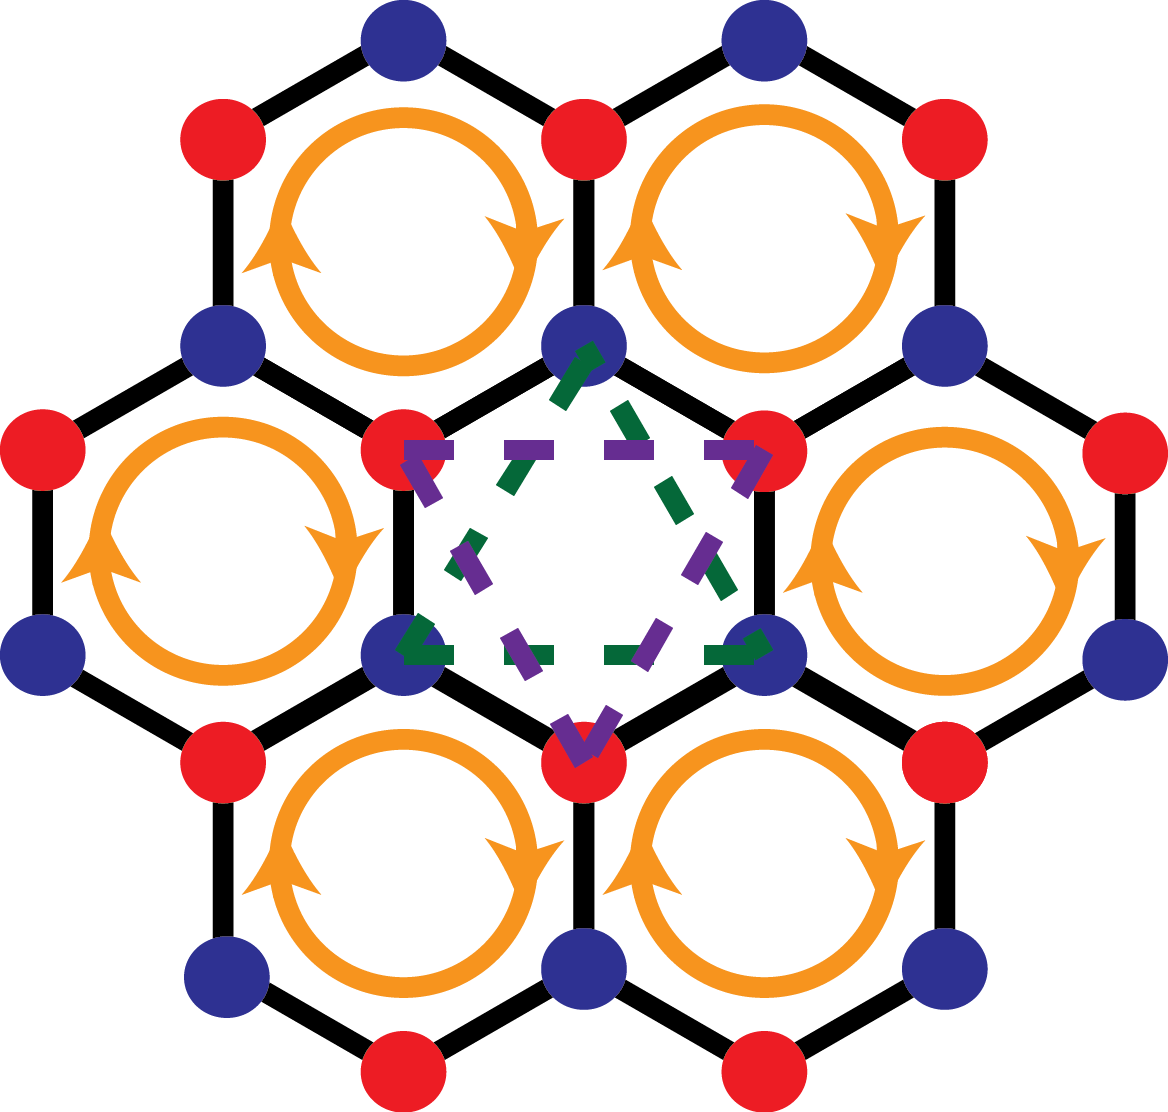
\includegraphics[width=40mm,keepaspectratio=true]{haldane_model.png}
\caption{The Haldane Model for Next Nearest Neighbor Hopping}\label{fig:haldane}
\end{figure}

\noindent Doing the same analysis as for the model in Eq. (\ref{eq:graphene_hamiltonian}),
\begin{align}
H|A,\vec{r} \rangle =
&-t \left( |B,\vec{r}+\vec{a}_1 \rangle + |B,\vec{r}+\vec{a}_2 \rangle + |B,\vec{r} \rangle \right) \notag \\
&- t' ( e^{i \alpha} |A,\vec{r}+\vec{a}_1 \rangle + e^{-i \alpha} |A,\vec{r}+\vec{a}_2 \rangle \, + \notag \\
&\qquad \, \, e^{i \alpha} |A,\vec{r}+\vec{a}_2 - \vec{a}_1 \rangle + e^{-i \alpha} |A,\vec{r} - \vec{a}_1 \rangle \, + \notag \\
&\qquad \, \, e^{i \alpha} |A,\vec{r}-\vec{a}_2 \rangle + e^{-i \alpha} |A,\vec{r} - \vec{a}_2 + \vec{a}_1 \rangle ) \\
H|B,\vec{r} \rangle =
&-t \left( |A,\vec{r}+\vec{a}_1 \rangle + |A,\vec{r}+\vec{a}_2 \rangle + |A,\vec{r} \rangle \right) \notag \\
&- t' ( e^{-i \alpha} |B,\vec{r}+\vec{a}_1 \rangle + e^{i \alpha} |B,\vec{r}+\vec{a}_2 \rangle \notag \, + \\
&\qquad \, \, e^{-i \alpha} |B,\vec{r}+\vec{a}_2 - \vec{a}_1 \rangle + e^{i \alpha} |B,\vec{r} - \vec{a}_1 \rangle \, + \notag \\
&\qquad \, \, e^{-i \alpha} |B,\vec{r}-\vec{a}_2 \rangle + e^{i \alpha} |B,\vec{r} - \vec{a}_2 + \vec{a}_1 \rangle )
\end{align}
Apply $H$ to the Bloch states defined in Eg. (\ref{eq:bloch_a}) and Eq. (\ref{eq:bloch_b}), and 
%\begin{align}
%H|A,\vec{k} \rangle =
%&-t \left( e^{-i \vec{k} \cdot \vec{a}_1} + e^{-i \vec{k} \cdot \vec{a}_2} +1 \right) |B,\vec{k} \rangle \notag \\
%&- t' ( e^{i \alpha} (  e^{-i \vec{k} \cdot \vec{a}_1} +  e^{-i \vec{k} \cdot (\vec{a}_2-\vec{a}_1)} +  e^{i \vec{k} \cdot %\vec{a}_2}) \, + \notag \\
%&\qquad \, \, e^{-i \alpha} (  e^{-i \vec{k} \cdot \vec{a}_2} +  e^{i \vec{k} \cdot (\vec{a}_2-\vec{a}_1)}  +  e^{i \vec{k} \cdot %\vec{a}_1})) |A,\vec{k} \rangle \\
%H|B,\vec{k} \rangle =
%&-t \left( e^{i \vec{k} \cdot \vec{a}_1} + e^{i \vec{k} \cdot \vec{a}_2} +1 \right) |A,\vec{k} \rangle \notag \\
%&- t' ( e^{i \alpha} (  e^{-i \vec{k} \cdot \vec{a}_2} +  e^{i \vec{k} \cdot (\vec{a}_2-\vec{a}_1)} +  e^{i \vec{k} \cdot \vec{a}_1}) \, + \notag \\
%&\qquad \, \, e^{-i \alpha} (  e^{-i \vec{k} \cdot \vec{a}_1} +  e^{-i \vec{k} \cdot (\vec{a}_2-\vec{a}_1)}  +  e^{i \vec{k} \cdot \vec{a}_2})) |B,\vec{k} \rangle
%\end{align}
define $S(\vec{k})=e^{i \vec{k} \cdot \vec{a}_1}+e^{i \vec{k} \cdot \vec{a}_2} +1$ and $T(\vec{k})=e^{-i \vec{k} \cdot \vec{a}_1} +  e^{-i \vec{k} \cdot (\vec{a}_2-\vec{a}_1)} +  e^{i \vec{k} \cdot \vec{a}_2}$.  Then, put $H$ in a matrix form
\begin{equation}
H(\vec{k})= \left(
\begin{array}{cc}
-t'[e^{i \alpha} T(\vec{k})+e^{-i \alpha} T^*(\vec{k})] & -tS^*(\vec{k}) \\
-tS(\vec{k}) & -t'[e^{-i \alpha} T(\vec{k})+e^{i \alpha} T^*(\vec{k})]
\end{array}
\right)
\end{equation}
Using $T(\vec{k}=\vec{K})=-\frac{3}{2}+\frac{3i \sqrt{3}}{2}$ and $S(\vec{k}=\vec{K}+\vec{q}) \approx -\frac{3}{2}a(q_x+i q_y)$
\begin{equation}
H(\vec{K}+\vec{q})= \left(
\begin{array}{cc}
3 \sqrt{3} t' \sin{\alpha} & 3at(q_x - i q_y)/2 \\
3at(q_x + i q_y)/2 & -3 \sqrt{3} t' \sin{\alpha}
\end{array}
\right)
\end{equation}
or expressed in terms of Pauli matrices
%\begin{equation}
%H(\vec{K}+\vec{q})=\hbar v_F (q_x \sigma_x + q_y \sigma_y)+(3 \sqrt{3} t' \sin{\alpha})\sigma_z
%\end{equation}
%A similar calculation shows that
%\begin{equation}
%H(\vec{K'}+\vec{q})=\hbar v_F (-q_x \sigma_x + q_y \sigma_y)+(-3 \sqrt{3} t' \sin{\alpha})\sigma_z
%\end{equation}
\begin{eqnarray}
H(\vec{K}+\vec{q})=\hbar v_F (q_x \sigma_x + q_y \sigma_y)+(3 \sqrt{3} t' \sin{\alpha})\sigma_z \\
H(\vec{K'}+\vec{q})=\hbar v_F (-q_x \sigma_x + q_y \sigma_y)+(-3 \sqrt{3} t' \sin{\alpha})\sigma_z
\end{eqnarray}
The coefficient of $\sigma_z$ is frequently referred to as the mass.  That the Haldane masses at $K$ and $K'$ have different sign is related to a lack of time reversal symmetry.

What is the Hall conductance?  For the trivial insulator, the mass terms at $K$ and $K'$ have the same sign, so by Eq. (\ref{eq:sign_of_mass}), the Hall conductance was zero.  For the Haldane mode, the masses at $K$ and $K'$ have opposite sign.  Thus, if $\sin{\alpha} \ne 0$, Eq. (\ref{eq:sign_of_mass}) implies that $\sigma_{xy}= \pm e^2/h$
%\begin{equation}
%\sigma_{xy}= \pm \frac{e^2}{h}
%\end{equation}
, where the sign of $\sigma_{xy}$ depends on the value of $\alpha$.

\end{section}

\begin{section}{The Edge State}

For both the Haldane model (henceforth referred to as a Haldane insulator) and the trivial insulator, we expanded the Hamiltonian matrix around $K$ and $K'$.  Whether we are near $K$ or $K'$ is called the ``valley" degree of freedom.  If we define $\tau_z$ as the third Pauli matrix acting on the valley degree of freedom (and $I$ as identity), we can unite the Hamiltonian expansions around $K$ and $K'$ into a single expression.  For the trivial insulator:
\begin{equation}
H=\hbar v_F (q_x \sigma_x \otimes \tau_z + q_y \sigma_y \otimes I) + U \sigma_z \otimes I
\end{equation}
and for the Haldane insulator:
\begin{equation}
H=\hbar v_F (q_x \sigma_x \otimes \tau_z + q_y \sigma_y \otimes I) + M_H \sigma_z \otimes \tau_z
\end{equation}
where $M_H=3 \sqrt{3} t' \sin{\alpha}$ is the Haldane mass.

Now, suppose we put a Haldane insulator next to a trivial insulator.  In the x-y plane, let $x<0$ be the trivial insulator and $x>0$ be the Haldane insulator.  We want to solve $H\Psi=E\Psi$.  Since we have translational symmetry in the y-direction, we can let $\Psi(x,y)=\psi(x) e^{ik_y y}$.  Also, for simplicity, let $\hbar v_F=1$ and $M=M_H=U$. Then \cite{dirac_materials}
\begin{equation}
\left[ -i \sigma_x \otimes \tau_z \partial / \partial x + q_y \sigma_y+M \left( \Theta(-x) \sigma_z+\Theta(x) \sigma_z \otimes \tau_z \right) \right] \psi(x)=E \psi(x)
\end{equation}
where $\Theta(x)$ is the Heaviside step function.  The identity matrix $I$ has been suppressed.  For the moment, lets look for mid-gap solutions by setting $q_y=0$ and $E=0$.

For $x>0$, $-i \sigma_x \otimes \tau_z \partial \psi / \partial x = -M \sigma_z \otimes \tau_z \psi$.  Multiply both sides by $i \sigma_z \otimes \tau_z$ to get $\partial \psi / \partial x = - M \sigma_y \psi$.  There exists two solutions to this differential equation that are localized on the boundary between the Haldane insulator and trivial insulator:
\begin{equation}
\psi_{\vec{K}}(x) = \frac{1}{\sqrt{2}} \left(
\begin{array}{c}
1 \\
i
\end{array}
\right) \otimes
\left(
\begin{array}{c}
1 \\
0
\end{array}
\right)
e^{- M |x|}, \text{ }
\psi_{\vec{K'}}(x) = \frac{1}{\sqrt{2}} \left(
\begin{array}{c}
1 \\
i
\end{array}
\right) \otimes
\left(
\begin{array}{c}
0 \\
1
\end{array}
\right)
e^{- M |x|}
\end{equation}
The corresponding differential equation for $x<0$ is $\partial \psi / \partial x = -M \sigma_y \otimes \tau_z \psi$.  Plugging both solutions into this equation reveals that only one of these solutions makes sense:
\begin{equation}
\psi_{\vec{K'}}(x) = \frac{1}{\sqrt{2}} \left(
\begin{array}{c}
1 \\
i
\end{array}
\right) \otimes
\left(
\begin{array}{c}
0 \\
1
\end{array}
\right)
e^{- M |x|}
\end{equation}
This solution is also an eigenvector of $q_y \sigma_y$, so we deduce that the energy-momentum dispersion relation for the edge state is $E=\hbar v_F q_y$, or allowing different signs of the Haldane mass at $K$,
\begin{equation}
E_{\text{Edge State}}=\text{sign}(M_H)\hbar v_F q_y
\label{eq:dispersion}
\end{equation}

\end{section}

\begin{section}{Winding Numbers}

What makes the Haldane insulator different from the trivial insulator?  Lets return to Eq. (\ref{eq:degree}), which can be written as
\begin{equation}
\sigma_{xy}=n \frac{e^2}{h}
\end{equation}
\begin{equation}
n=\frac{1}{4 \pi} \int_{BZ} \hat{\vec{d}}(\vec{k}) \cdot \left( \frac{\partial \hat{\vec{d}}(\vec{k})}{\partial k_x} \times \frac{\partial \hat{\vec{d}}(\vec{k})}{\partial k_y}\right) dk_x dk_y
\label{eq:winding}
\end{equation}
where $\hat{\vec{d}}(\vec{k})=\vec{d}(\vec{k})/|\vec{d}(\vec{k})|$ is the unit vector in the $\vec{d}(\vec{k})$ direction, and $n$ is an integer that goes by many names: the degree of continuous mapping, the first Chern number, the TKNN invariant, and the winding number \cite{hasan_kane_review}.  The image of the map $\vec{k} \rightarrow \vec{d}(\vec{k})$ is a closed surface (denoted $S$) embedded in $\mathbb{R}^3$.  The winding number $n$ is the number of times $S$ encloses the origin:
\begin{equation}
n= \frac{1}{4 \pi} \int_{BZ} \frac{\vec{d}(\vec{k})}{|\vec{d}(\vec{k})|^3}\cdot \left( \frac{\partial \vec{d}(\vec{k})}{\partial k_x} \times \frac{\partial \vec{d}(\vec{k})}{\partial k_y}\right) dk_x dk_y = \int_S \frac{\hat{\vec{d}}(\vec{k})}{4 \pi |\vec{d}(\vec{k})|^2} \cdot d\vec{S}
\end{equation}
This familiar integral is just the flux of a monopole centered at the origin.  If $S$ does not enclose the origin, $n=0$.  If $S$ encloses the origin once, $n=1$ (or $n=-1$ depending on the orientation of $S$, but we will not worry about orientation), and so on.

%Here is a helpful way to visualize the surface $S$.  The Hamiltonian $H=\vec{d}(\vec{k}) \cdot \vec{\sigma}$ looks just like a spin 1/2 particle in a magnetic field $\vec{d}(\vec{k})$ and with energy $E=\pm |\vec{d}(\vec{k})|$.  Every electron in our insulator experiences a different ``pseudo-magnetic field" $\vec{d}(\vec{k})=(d_x,d_y,d_z)$.  Now, imagine an x-y-z coordinate system.  Put each electron at $(d_x,d_y,d_z)$ on the x-y-z coordinate system.  No electron will sit on the origin $(0,0,0)$ because we have an insulator.  The electrons will form the closed surface $S$ that either does or does not enclose the origin.  In a moment, we will see that the trivial insulator does not enclose the origin whereas the Haldane insulator does.

The trivial insulator has Hamiltonian $H=\xi q_x \sigma_x + q_y \sigma_y + M \sigma_z$, where $\xi=1$ for $K$ and $\xi=-1$ for $K'$.  If $M$ is positive, then the vector $\vec{d}(\vec{k})$ lies on the positive z-axis of $\mathbb{R}^3$ (the north pole) at $K$ and $K'$.  It is easy to see that $\vec{d}(\vec{k})$ does not lie on the z-axis for any other $\vec{k}$.  What surface $S$ crosses the north pole twice but never crosses the south pole (the negative z-axis)?  The surface $S$ clearly does not enclose the origin, and thus $n=0$ and $\sigma_{xy}=0$.

The Haldane insulator has Hamiltonian $H=\xi q_x \sigma_x + q_y \sigma_y + \xi M \sigma_z$.  Now, $\vec{d}(\vec{K})=(0,0,M)$, $\vec{d}(\vec{K'})=(0,0,-M)$, and $(d_x, d_y) \ne (0,0)$ everywhere else in the Brillouin zone.  Thus, the surface $S$ crosses the north pole once and the south pole once.  A closed surface that crosses the north and south pole each exactly once must contain the origin exactly one time!  We conclude that $|n|=1$ and $|\sigma_{xy}|=1$.

Now, suppose we adiabatically evolved the Haldane insulator into the trivial insulator.  
%That is equivalent to deforming the surface $S$ for the Haldane insulator into the surface for the trivial insulator.
In order to continuously deform a surface that encloses the origin into a surface that does not enclose the origin, the surface must cross the origin.  This implies that $\vec{d}(\vec{k})=0$ at some point during the adiabatic evolution, so the energy gap closes!  We would say that the Haldane insulator and trivial insulator are different topological phases.  This is why we have a conducting edge state when we put a Haldane insulator and trivial insulator next to each other.  When you cross the boundary between the two insulators, the gap must close.

\end{section}

\begin{section}{The Kane and Mele Model}

Now we finally introduce a model for the quantum spin Hall (QSH) effect.  Kane and Mele proposed the following Hamiltonian for a honeycomb lattice with spin-orbit coupling \cite{kane_mele_prl}
\begin{equation}
\label{eq:kane_and_mele}
H= \left[ - t \sum_{\langle i,j \rangle \alpha} a_{i \alpha}^\dagger b_{\alpha j} - i t' \sum_{\langle \langle i,j \rangle \rangle} \nu_{ij} \left( s_z \right)_{\alpha \beta} a_{i \alpha}^\dagger a_{j \beta} - i t' \sum_{\langle \langle i,j \rangle \rangle \alpha \beta} \nu_{ij} \left( s_z \right)_{\alpha \beta} b_{i \alpha}^\dagger b_{j \beta} \right] + \text{h.c.}
\end{equation}
where $s_z$ is the third Pauli matrix acting on the spin degree of freedom, $\alpha$ and $\beta$ are spin indices (up and down), and $\nu_{ij}=\pm 1$ depending on whether the electron hops clockwise or counterclockwise to its next nearest neighbor.

The Kane and Mele Hamiltonian is just two copies of the Haldane model, with $\alpha=\pi/2$ for spin up and $\alpha=-\pi/2$ for spin down.  Therefore, we can rewrite Eq. (\ref{eq:kane_and_mele}) as
\begin{equation}
H=\hbar v_F (q_x \sigma_x \otimes \tau_z + q_y \sigma_y)+\Delta_{SO} \sigma_z \otimes \tau_z \otimes s_z
\end{equation}
where $\Delta_{SO}=3 \sqrt{3} t'$.  Since the mass term is positive for spin up and negative for spin down, Eq. (\ref{eq:dispersion}) implies that there are two counter-propagating edge modes.  The spin of an edge mode is locked to its momentum (spin up for $+q_y$, spin down for $-q_y$%, see Fig. \ref{fig:qsh_edges}
).  This had to be true because the Kane and Mele model (unlike the Haldane model) obeys time reversal symmetry and therefore has a Kramers degeneracy.

%\begin{figure}[h!]
%\centering
%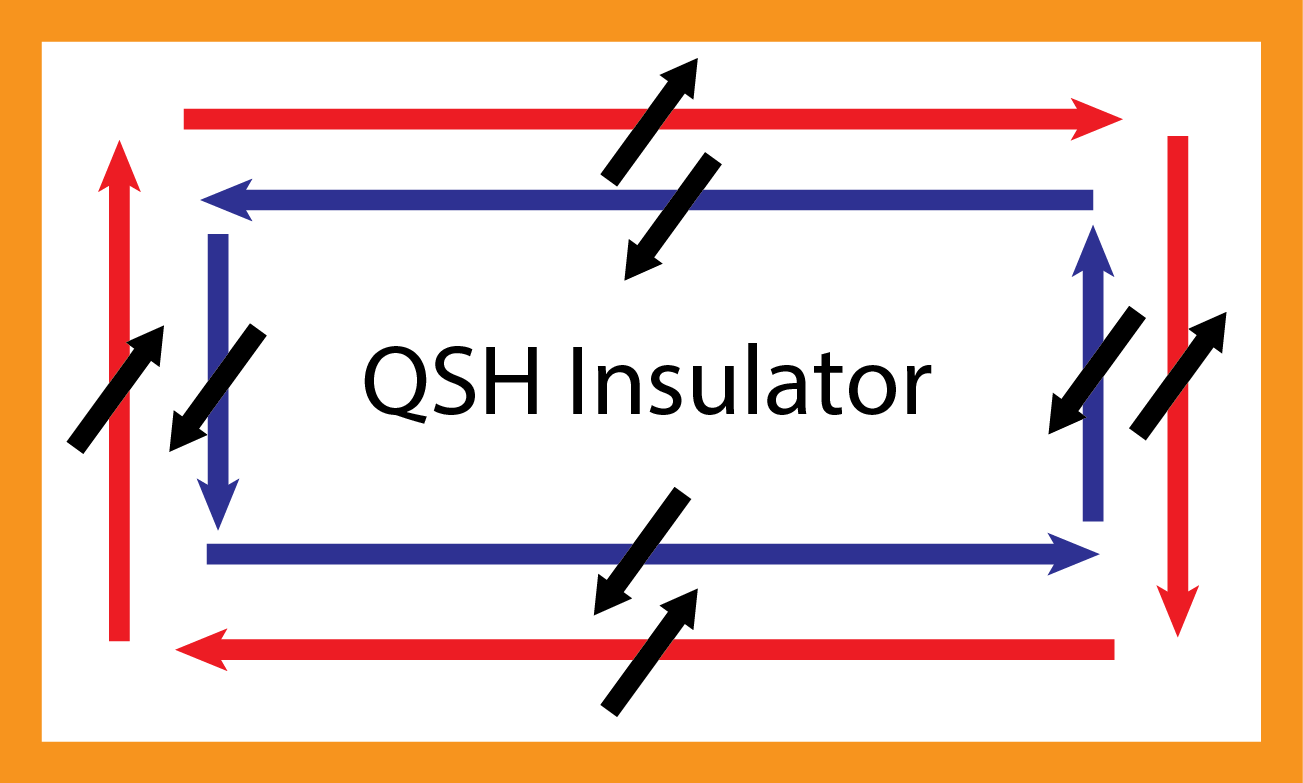
\includegraphics[width=50mm,keepaspectratio=true]{qsh_edges.png}
%\caption{Helical Edge States of a Quantum Spin Hall Insulator}\label{fig:qsh_edges}
%\end{figure}

The winding numbers for spin up and spin down have opposite sign, so total $\sigma_{xy}=0$.  However, the Kane and Mele model is still different from the trivial insulator because we can define a new topological invariant: the spin Chern number $C_{spin}=(n_\uparrow-n_\downarrow)/2$, where $n_\uparrow$ and $n_\downarrow$ are the winding numbers for spin up and down, respectively.  The spin Chern number describes the spin current, which is nonzero because spin and momentum are locked.  The Kane and Mele model of a QSH insulator has $|C_{spin}|=1$.

An astute reader will notice that the Kane and Mele model conserves $s_z$, which may not happen with a different spin-orbit coupling term.  The actual topological invariant that characterizes time reversal symmetric insulators is the so-called $\mathbb{Z}_2$ invariant, which takes values 0 (for the trivial phase) and 1 (for the nontrivial phase) \cite{kane_mele_z2}.  If $s_z$ is conserved, the $\mathbb{Z}_2$ invariant is equal to $C_{spin} \text{ mod } 2$.  We will not define the $\mathbb{Z}_2$ invariant more generally because it requires additional mathematical machinery, such as the Pfaffian of a matrix.  Although it is too long to include in this paper, the theory of the $\mathbb{Z}_2$ invariant is quite interesting and describes the inability to define a smooth gauge convention that obeys time reversal symmetry.  We will also note that, for systems with inversion symmetry, the $\mathbb{Z}_2$ invariant can be calculated through some product of parity eigenvalues at certain high symmetry points in the Brillouin zone (specifically $\vec{k}$ that are mapped onto themselves under time reversal) \cite{fu_inversion}.

\end{section}

\begin{section}{Protection from Backscattering}

Even without discussing the $\mathbb{Z}_2$ invariant, we can give a heuristic argument for the protection of the QSH edge states \cite{sun_kai}.  As long as the bulk remains gapped, time reversal symmetric perturbations cannot gap the edge states.  If we define $k=q_y$ in Eq. (\ref{eq:dispersion}), then $E_{edge, \alpha} = (s_z)_{\alpha \alpha} \hbar v_F k$.  We can write a Hamiltonian just for the edge modes
\begin{equation}
H=\hbar \left(
\begin{array}{cc}
v_F k & 0  \\
0 & -v_F k
\end{array}
\right)
\end{equation}
A pair of counter-propagating edge modes is called a Dirac cone.  The two edge states meet at the ``Dirac point" at $k=0$.  If we apply a time reversal symmetric perturbation, will the two edge states still cross at the Dirac point?  The most general time reversal symmetric perturbation that we can write is
\begin{equation}
H'=\sum_{ni} \left[ a_{ni} k^{2n+1} s_i + b_n k^{2n} I  \right]
\end{equation}
where $s_i$ are the three Pauli matrices and $I$ is the identity matrix.  At $k=0$, $H'=b_0 I$, so the two edge modes are still degenerate at $k=0$.  Therefore, no gap opens, and the edge states remain metallic.  This would not be true if $H'$ disobeyed time reversal symmetry.

Suppose we had two copies of the Kane and Mele model.  If we had two Dirac cones, would our metallic edge states be protected by time reversal symmetry?  We can represent two Dirac cones by the Hamiltonian
\begin{equation}
H=
\hbar \left(
\begin{array}{cc}
v_1 k & 0  \\
0 & -v_1 k
\end{array}
\right)
\oplus
\left(
\begin{array}{cc}
v_2 k & 0  \\
0 & -v_2 k
\end{array}
\right)
=\hbar \left(
\begin{array}{cccc}
v_1 k & 0 & 0 & 0 \\
0 & -v_1 k & 0 & 0 \\
0 & 0 & v_2 k & 0 \\
0 & 0 & 0 & -v_2 k
\end{array}
\right)
\end{equation}
where $v_1$ and $v_2$ are the velocities of the edge states.  For simplicity, we will consider the case $v_F=v_1=v_2$.  We can express the time reversal operator as $UK$, where $K$ takes numbers to their complex conjugates, and $U$ is given by
\begin{equation}
U=
\left(
\begin{array}{cc}
0 & 1  \\
-1 & 0
\end{array}
\right)
\oplus
\left(
\begin{array}{cc}
0 & 1  \\
-1 & 0
\end{array}
\right)
=\left(
\begin{array}{cccc}
0 & 1 & 0 & 0\\
-1 & 0 & 0 & 0 \\
0 & 0 & 0 & 1 \\
0 & 0 & -1 & 0
\end{array}
\right)
\end{equation}
Now, lets consider a particular perturbation of the system
\begin{equation}
H'
=\left(
\begin{array}{cccc}
0 & 0 & 0 & \lambda \\
0 & 0 & -\lambda & 0 \\
0 & -\lambda & 0 & 0 \\
\lambda & 0 & 0 & 0
\end{array}
\right)
\end{equation}
It is easy to check that $(UH'U^{-1})^*=H'$, so $H'$ is time reversal symmetric.  However, if we diagonalize the full Hamiltonian $H+H'$, we get the energy eigenvalues $E=\pm \sqrt{(\hbar v_F k)^2+\lambda^2}$.  Thus, the edge states become gapped by the perturbation.

More generally, time reversal symmetric perturbations destroy pairs of Dirac cones.  Therefore, if there are an odd number of Dirac cones, the metallic edge states are protected against time reversal invariant perturbations.  If there are an even number of Dirac cones, these edge modes are not protected.  Since the Kane and Mele QSH insulator has one Dirac cone, its edge channels are robust, so long as the bulk remains gapped.

\end{section}

%\begin{section}{Experimental Evidence}
%
%
%\end{section}
%
%\begin{section}{Summary}
%
%
%\end{section}

\begin{thebibliography}{1}

\singlespacing
\footnotesize

\bibitem{griffiths} D. J. Griffiths, {\em Introduction to Quantum Mechanics} (2004)
\bibitem{bernevig} B. A. Bernevig and T. L. Hughes, {\em Topological Insulators and Topological Superconductors} (2013)
\bibitem{louie} Cohen and Louie, Chapter 5
\bibitem{luttinger} R. Karplus and J. M. Luttinger, {\em Physical Review} \textbf{95}, 1154 (1954).
\bibitem{tknn} D. J. Thouless, M. Kohmoto, M. P. Nightingale, M. den Nijs, {\em Physical Review Letter} \textbf{49}, 405 (1982)
\bibitem{berry_electronic} D. Xiao, M. C. Chang, and Q. Niu, {\em Reviews of Modern Physics} \textbf{82}, 1959 (2010)
\bibitem{katsnelson} M. I. Katsnelson, {\em Graphene: Carbon in Two Dimensions} (2012)
\bibitem{castro_neto} A. H. Castro Neto, F. Guinea, N. M. R. Peres, K. S. Novoselov, A. K. Geim, {\em Reviews of Modern Physics} \textbf{81}, 109 (2009)
\bibitem{dirac_materials} J. Cayssol, {\em Comptes Rendus Physique} \textbf{14} 760-778 (2013)
\bibitem{haldane_prl} F. D. M. Haldane, {\em Physical Review Letters} \textbf{61}, 2015 (1988)
\bibitem{hasan_kane_review} M. Z. Hasan and C. L. Kane, {\em Reviews Modern Physics} \textbf{82}, 3045 (2010)
\bibitem{kane_mele_prl} C. L. Kane and E. J. Mele, {\em Physical Review Letters} \textbf{95}, 226801 (2005)
\bibitem{kane_mele_z2} C. L. Kane and E. J. Mele, {\em Physical Review Letters} \textbf{95}, 146802 (2005)
\bibitem{fu_inversion} Liang Fu and C. L. Kane {\em Physical Review B} \textbf{76}, 045302 (2007)
\bibitem{sun_kai} Sun Kai's lecture notes, University of Michigan
\bibitem{zhang} B. A. Bernevig, T. L. Hughes, S. C. Zhang, {\em Science} \textbf{314} 1757 (2006)
\bibitem{konig} M. K\"onig {\em et al}., {\em Science} \textbf{318}, 766 (2007)
\bibitem{annual_review} J. Maciejko, T. L. Hughes, S. C. Zhang, {\em Annual Review of Condensed Matter Physics} \textbf{2} 31 (2011)
\bibitem{brune} C. Br\"une {\em et al}., {\em Nature Physics} \textbf{8}, 485 (2012)
\bibitem{fu_3d} Liang Fu, C. L. Kane, and E. J. Mele {\em Physical Review Letters} \textbf{98}, 106803 (2007)
\bibitem{hasan} D. Hsieh {\em et al}., {\em Nature} \textbf{452}, 970 (2008)
\bibitem{spintex} D. Hsieh {\em et al}., {\em Science} \textbf{323}, 919 (2009)
\bibitem{yazdani} P. Roushan {\em et al}., {\em Nature} \textbf{460}, 1106 (2009)
\bibitem{zx_shen} Y. L. Chen {\em et al}., {\em Science} \textbf{325}, 178 (2009)
\bibitem{massive_zx_shen} Y. L. Chen {\em et al}., {\em Science} \textbf{329}, 659 (2010)
\bibitem{qah} C. Z. Chang {\em et al}., {\em Science} \textbf{340}, 167 (2013)
\bibitem{dirac_semimetal} Z. K. Liu {\em et al}., {\em Science} \textbf{343}, 864 (2014)

\end{thebibliography}

\end{document}